\chapter{Apéndice}
\section{Proceso de escritura en memoria}  \label{writing_subsecc}

Se analiza el caso de tener instanciadas $N=4$, $MACs$ y un kernel con $k=3$
para clarificar la operación del algoritmo descrito. El proceso de escritura en
memoria, utilizando el desplazamiento circular de columnas mencionado.

Como consideramos un kernel con $k=3$ y $N=4$, $MACs$:
	    
\begin{itemize}
\item Se necesitan o requieren N+k-1=4+3-1=6 columnas de memoria
\item En la primera iteración, se cargan las memorias 1 a 6 con el nuevo lote
  (donde cada memoria instanciada alberga una columna del lote) y el resultado
  se almacena en las memorias 1 a 4, marcadas con otro color y en la etapa run
  out.
\item En la segunda iteración, los datos del nuevo lote se cargan sin
  sobrescribir las memorias 5 y 6 . Luego del procesamiento, se almacenan los
  datos comenzando en la memoria  5 hasta la última, para luego sobrescribir los
  datos del lote previo desde el principio.
\end{itemize}

Lo anterior se puede apreciar en la figura~\ref{writingprocess1}, donde se
incluye una línea punteada que separa la etapa de carga y la de procesamiento y
salida de dato

\begin{figure}
\centering
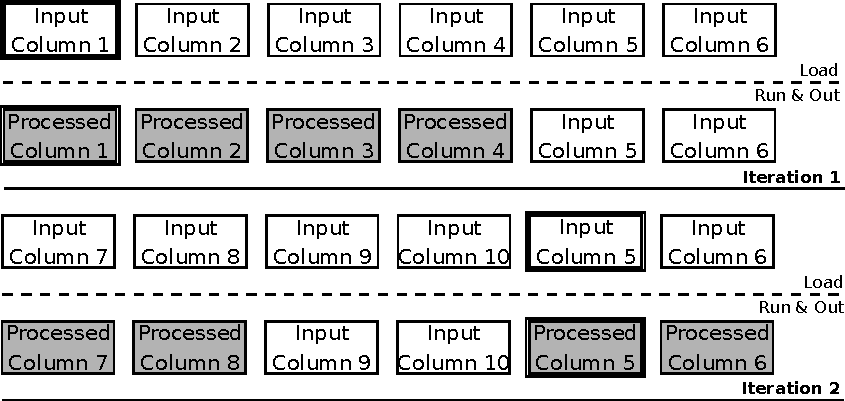
\includegraphics[scale=0.8]{algorithm}
\caption{Algoritmo de escritura para N=4, k=3 }
\label{writingprocess1}
\end{figure}

Considerando ahora un kernel con $k=3$ y  $N=2$, $MACs$, las
figuras~\ref{writingprocess2} y~\ref{writ_proc} intentan ilustrar lo mencionado
de forma mas clara, donde se distinguen con colores las columnas involucradas y
las etapas respectivas.

\begin{figure}
\centering
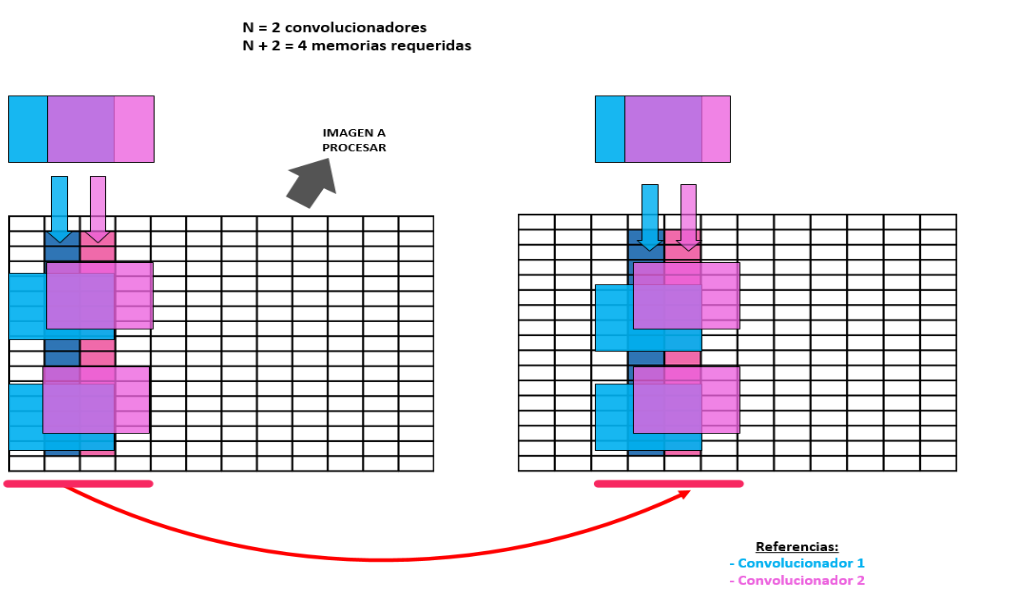
\includegraphics[scale=0.75]{conv2_despl.png}
\caption{Desplazamiento del kernel para N=2, k=3 }
\label{writingprocess2}
\end{figure}

% \begin{figure}
% \centering
% 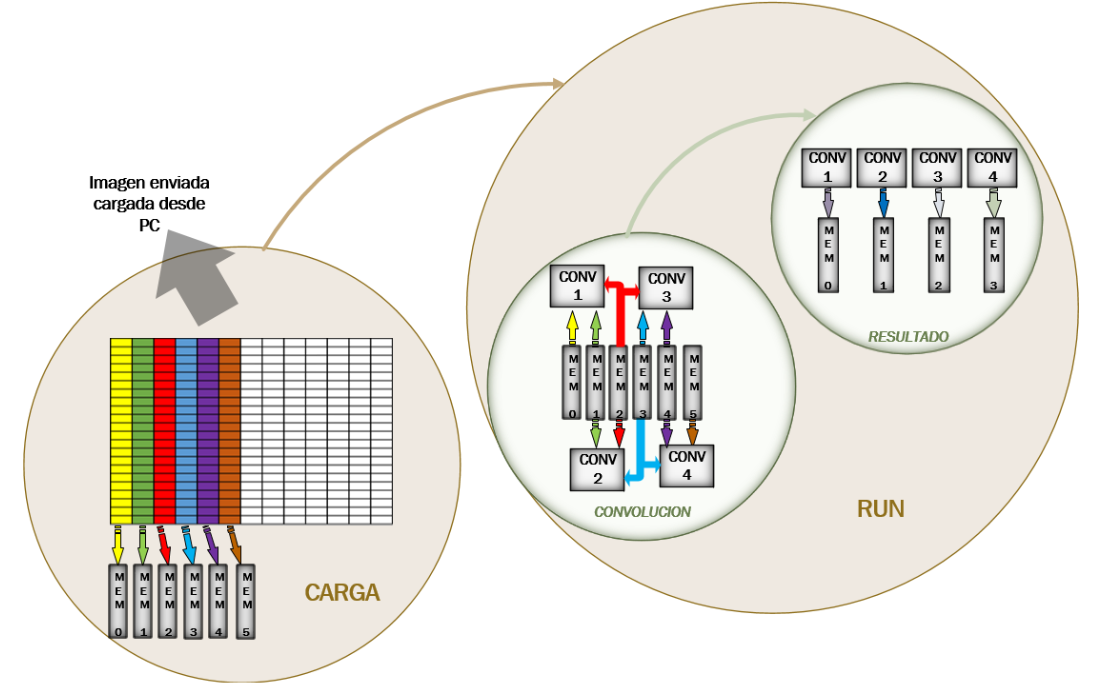
\includegraphics[scale=0.5]{example_1}
% \caption{Primera iteración con N=2, k=3 }
% \label{writingprocess3}
% \end{figure}


% \begin{figure}
% \centering
% 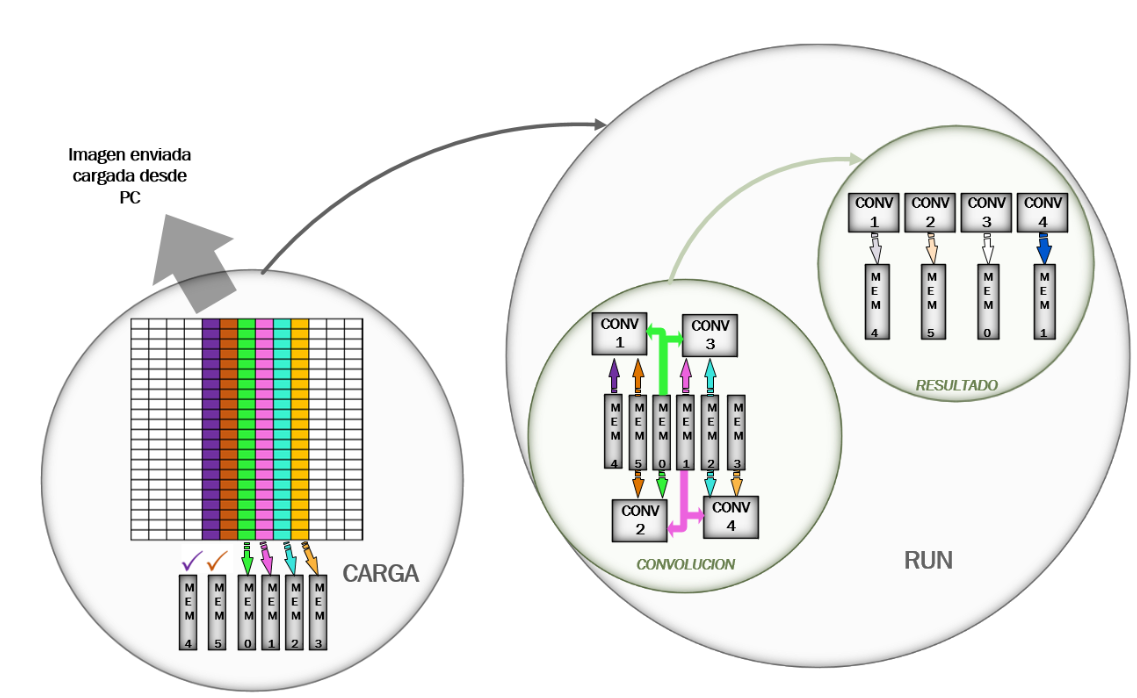
\includegraphics[scale=0.5]{example_2}
% \caption{Siguiente iteración con N=2, k=3}
% \label{writingprocess4}
% \end{figure}

\begin{figure}[!t]
\centering
\subfloat[][Primera iteración]{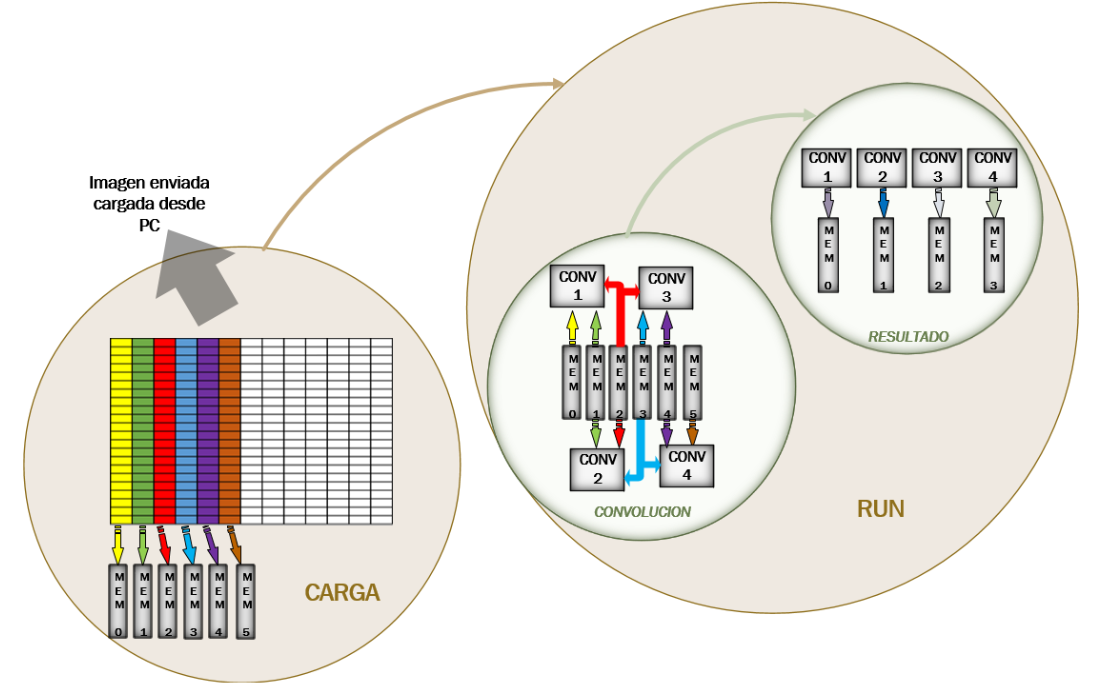
\includegraphics[scale=0.5]{example_1}}
\hfil
\subfloat[][Iteración siguiente]{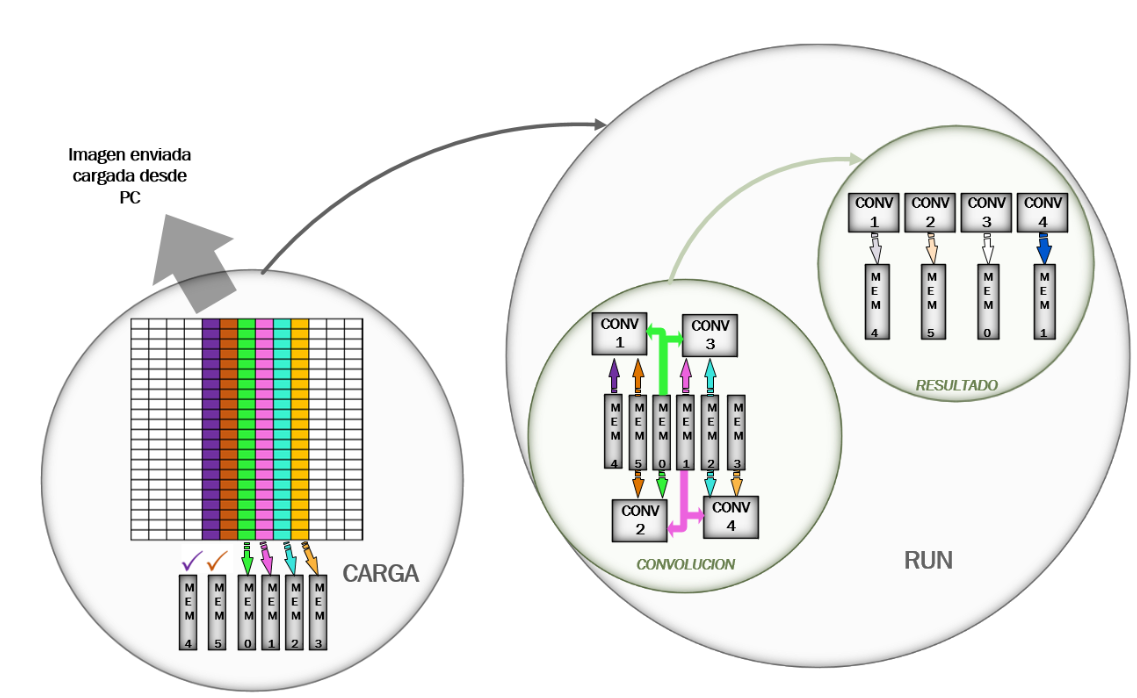
\includegraphics[scale=0.5]{example_2}}
\caption{Escritura y lectura de memorias para $N=2$, $k=3$.}
\label{writ_proc}
\end{figure}
% \clearpage
% \newpage
